\subsection{Colombia}\label{subsec:col}

\subsection*{Detector Description}

Colombia WCD, Guane-3, share similar characteristics with other LAGO WCDs.
Located at Bucaramanga in the Universidad Industrial of Santander, it is a
cylindrical reservoir filled with high quality purified water up to a level of
55 cm, and 103 cm of radio, and with a area of detection of 2.61m$^2$. The
water is contained in a reflective and diffusive bag, made of
Tyvek$^{\textregistered}$. The water volume is overlooked by a single Hamamatsu
photomultiplier tube of 8'' with a 25\% efficiency at 400\,nm. A picture of the
detector is showed in Fig. \ref{fig:Guane3WCD}. The electronics is the same
developed by the Bariloche group. 

\begin{figure}[h!]
\begin{center}
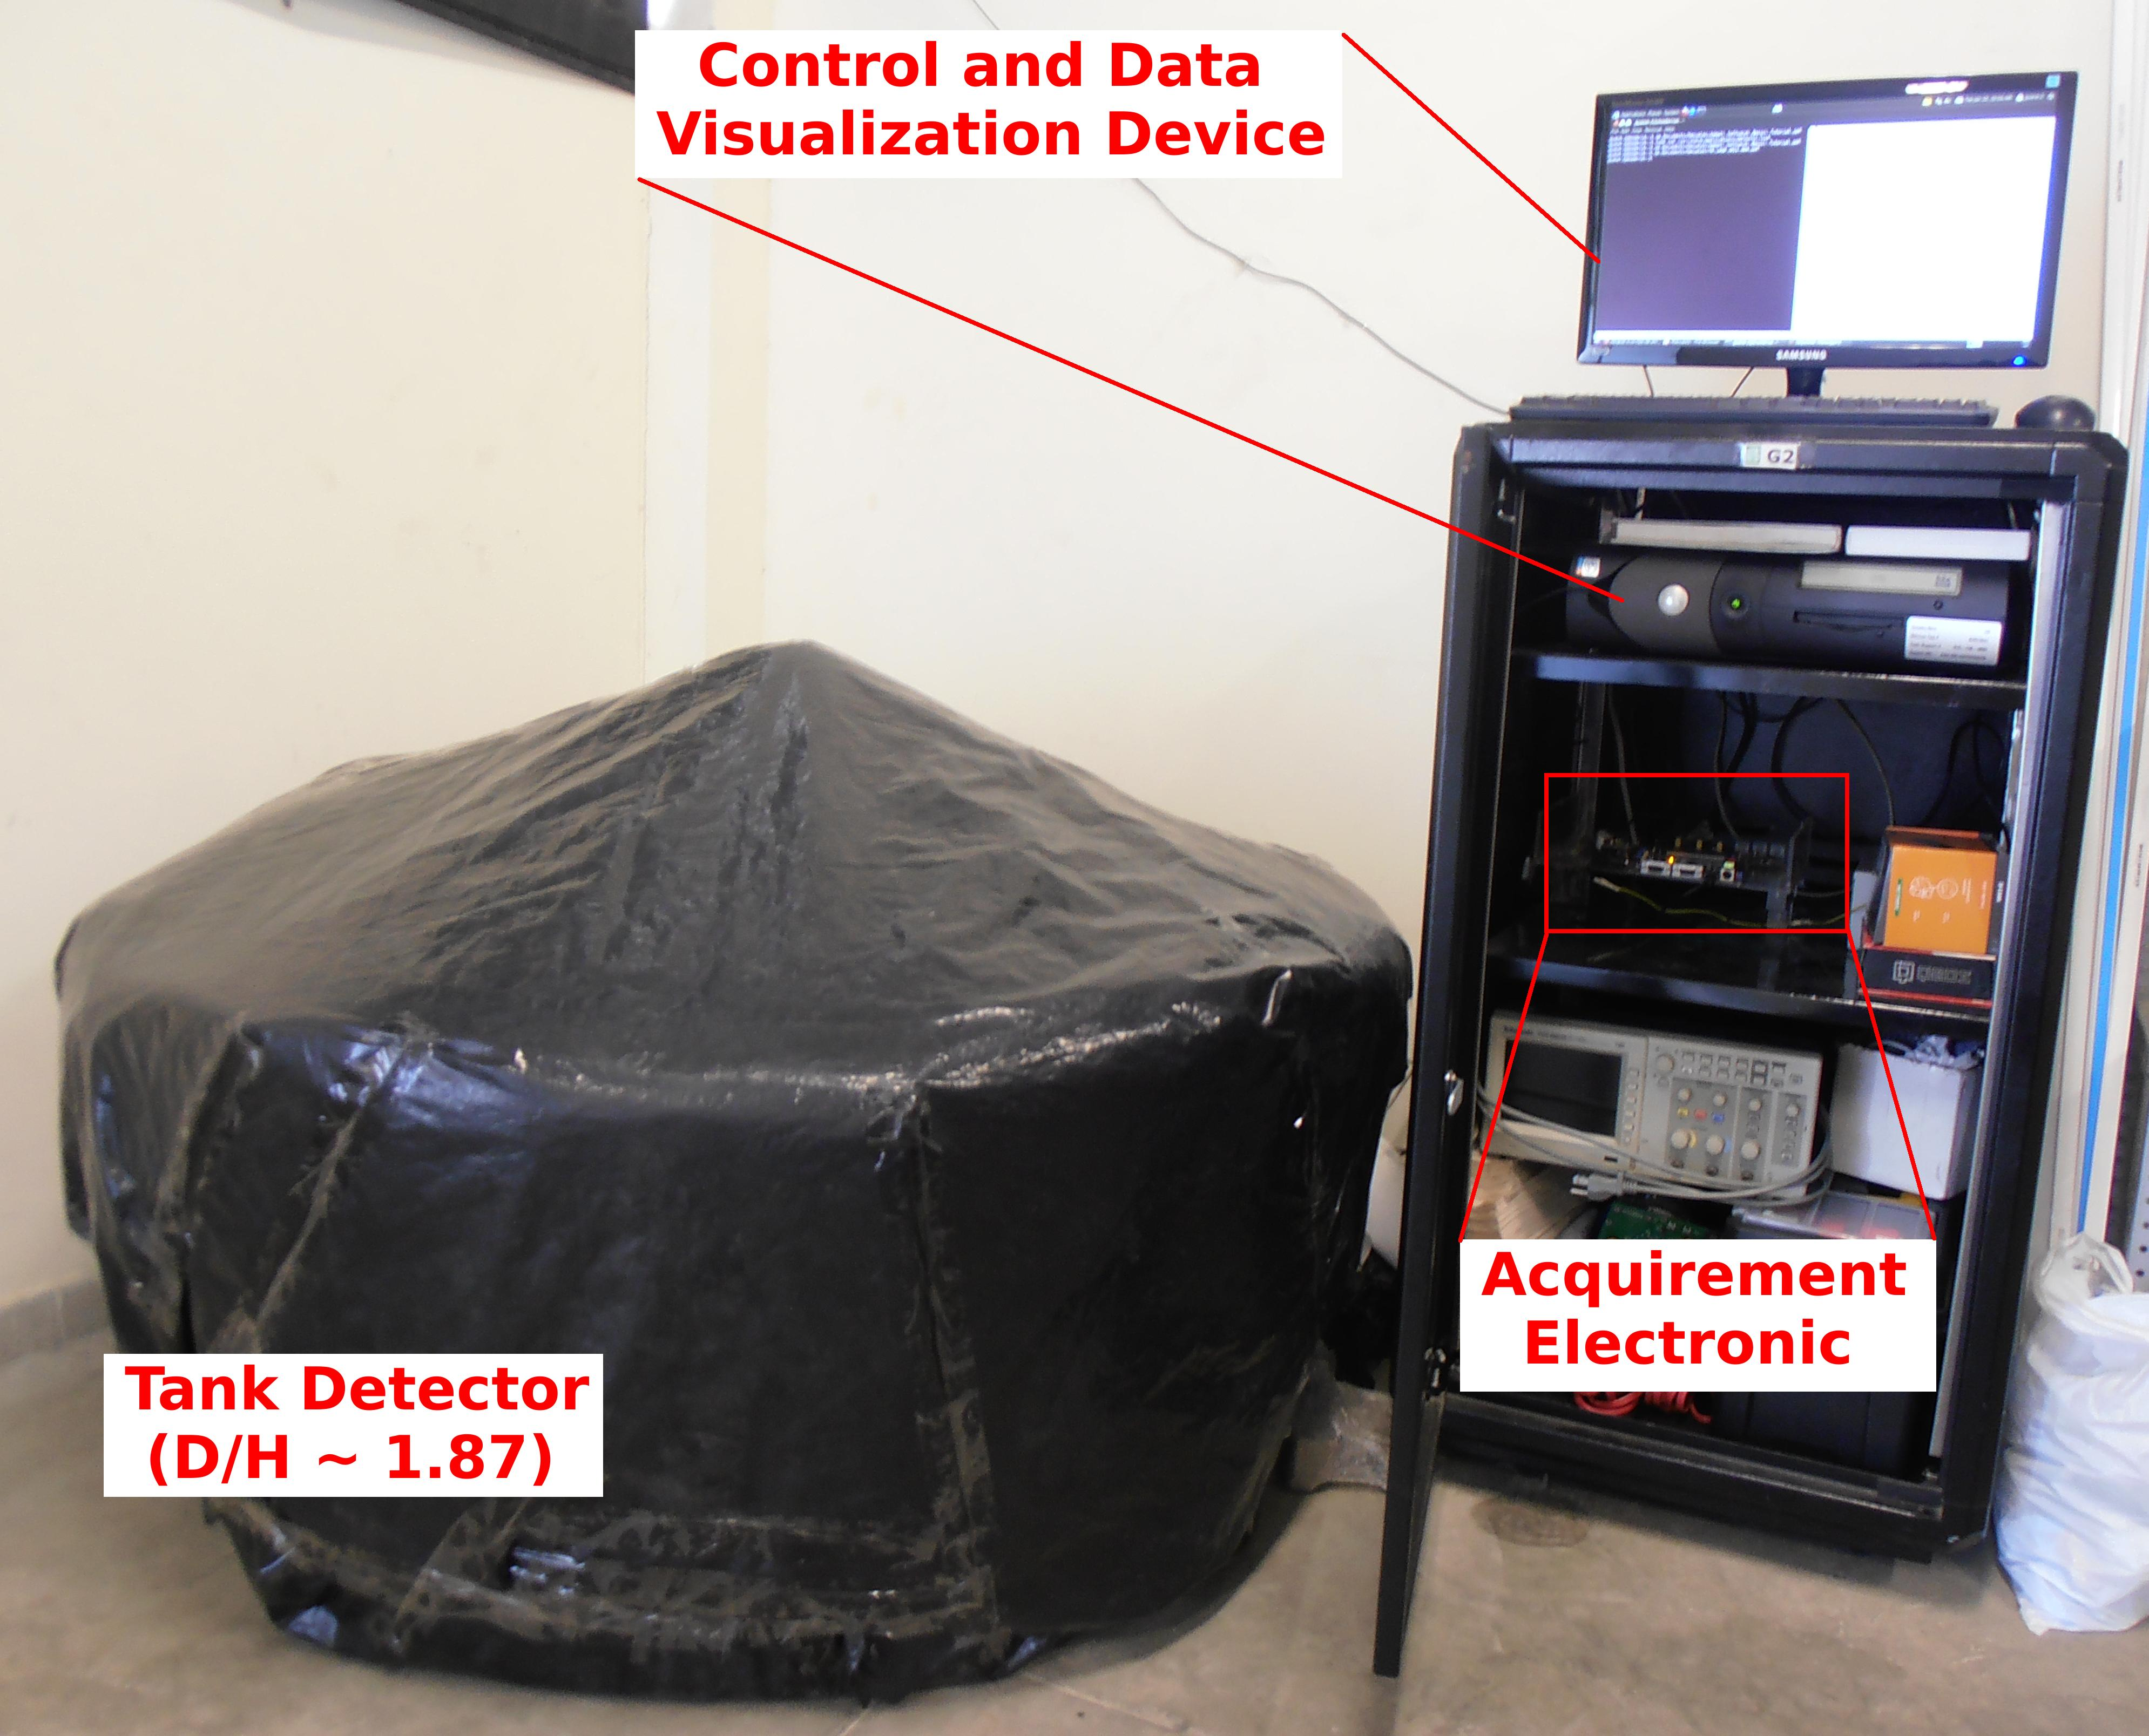
\includegraphics[width=3in]{images/colombia/WCD-Guane3.jpg}
\caption{GUANE-3 WCD at Bucaramanga.}
\label{fig:Guane3WCD}
\end{center}
\end{figure}

From fig. \ref{fig:results-col}, right, can be appretiated pulses registered by
Guane-3 having a particular shape: rapid increase and declining exponentially.

\begin{figure}
\centering
%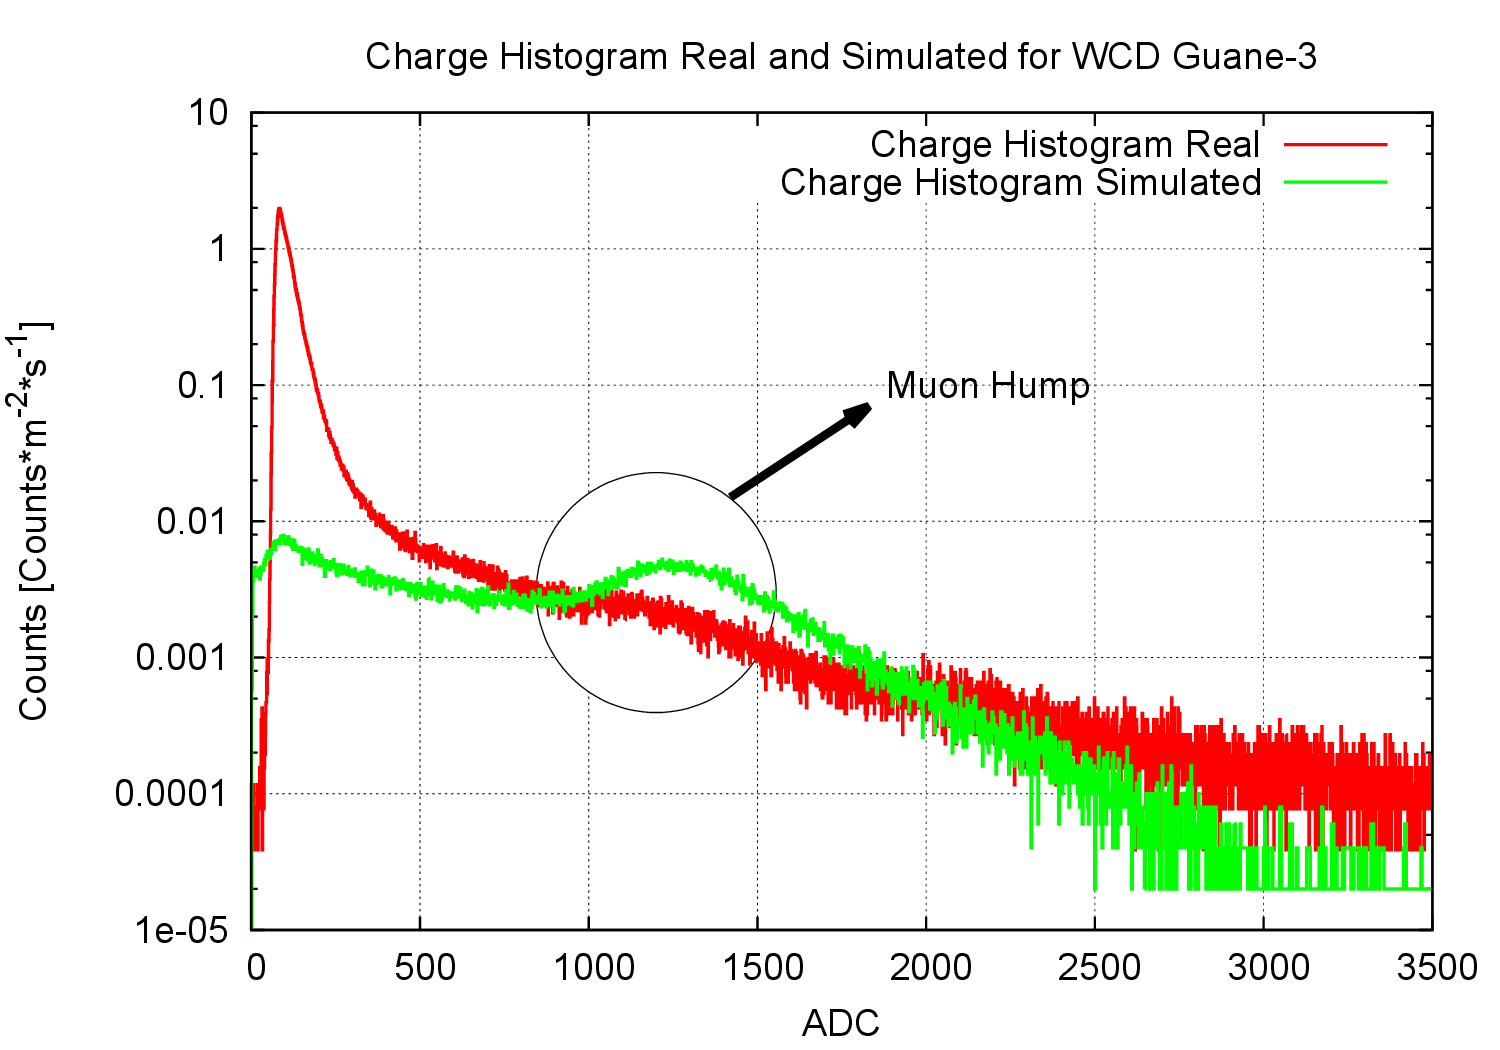
\includegraphics[width=0.49\textwidth]{images/colombia/Histcharge-Guane3.png}
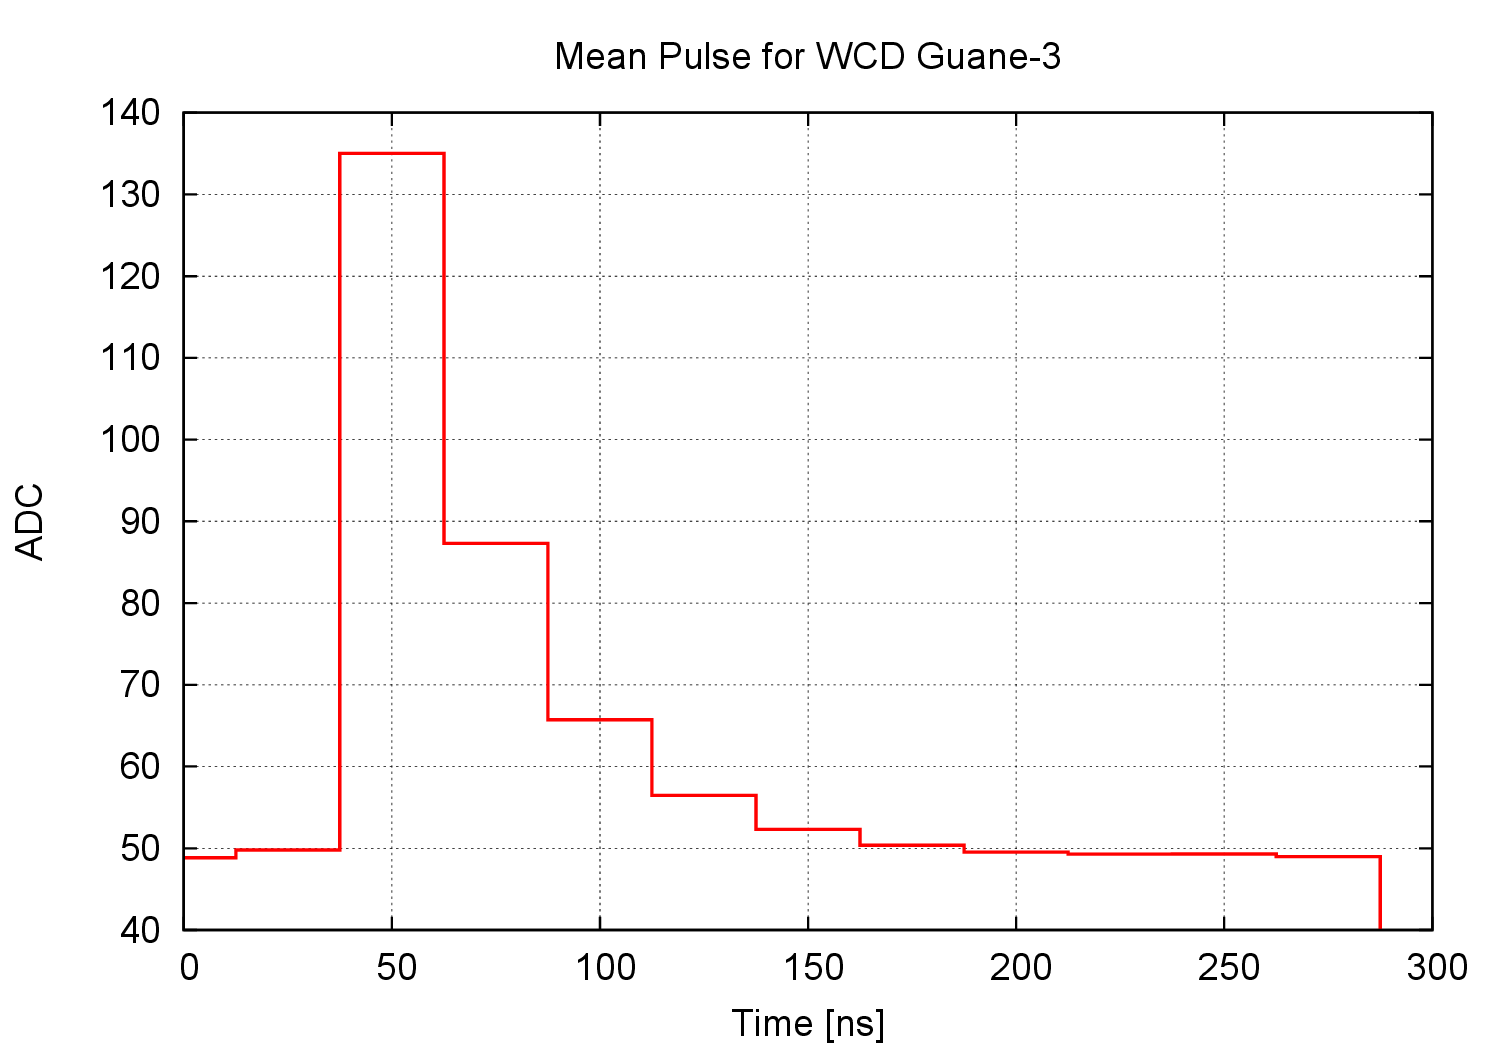
\includegraphics[width=0.49\textwidth]{images/colombia/MeanPulse-Guane3.png} 
\caption{Left: simulated and real charge histogram for the GUANE-3 WCD. Right: a plot of the mean pulse is depicted.} 
\label{fig:results-col}
\end{figure}

Calibrating, operating and monitoring WCDs at high altitude or remote
countryside places can be a significant complex task. The characteristic hump
left by muons in a WCD (such as the one used for calibrating the Pierre Auger
Observatory WCDs, see \cite{Bertou2006} is smeared by the large background
of electrons, positrons and photons. In order to calibrate Guane-3 WCD, it is
standard to use the VEM \cite{Etchegoyen2005}. Thus this unit defines the
high energy region ($>$1 VEM) and the low energy region ($<$1 VEM). The
equivalence between VEM and ADC units, can be obtained by comparing the charge
histograms with the corresponding Montecarlo simulations. For our Guane-3 WCD
we have 1 VEM $\sim 1200$ ADC. 


%seria bueno poner un grafico de esta calibracion!

